\chapter{Realization}

In the following chapter, we describe the realization of the software system. In section \ref{sec:structure}, we give an overview of the different components and how they interact with each other. In section \ref{sec:changes}, we list the changes which have to be made to existing components.

\section{Structure}\label{sec:structure}

The system consists of three major components: the \emph{Social Bot}, the \emph{Mensa Service} and the \emph{MobSOS CCA} backend service.

The MobSOS CCA backend service has access to three different databases. First, the MobSOS CCA service can access the food reviews, which are stored inside the las2peer database of the Mensa Service. Second, the system can access \emph{Mediabase} data, which contains data from reviews, made outside of the las2peer system. This data will be collected by a crawler bot, which searches Google and Twitter for reviews of the canteen. Those two databases provide the information quality factors of the MobSOS success model.
Third, the CCA service can also access monitoring data generated by the Bot and the Mensa Service. Those monitoring messages provide the system quality factors of the MobSOS success model.

The Bot Service acts as an interface between the user, and the backend services Mensa Service and CCA service.
The Bot Service communicates with the \emph{Mensa Service} in order to get the menu for the canteen. Additionally, the bot can send requests to the Mensa service, telling it to add, or modify, reviews.

The Bot Service communicates with the CCA system in order to retrieve data and visualisations of the success model. Furthermore, the MobSOS CCA system can also be used to modify the success model of the system. The bot sends the visualisations to the user in chat.

\begin{figure}[h]
  \centering
  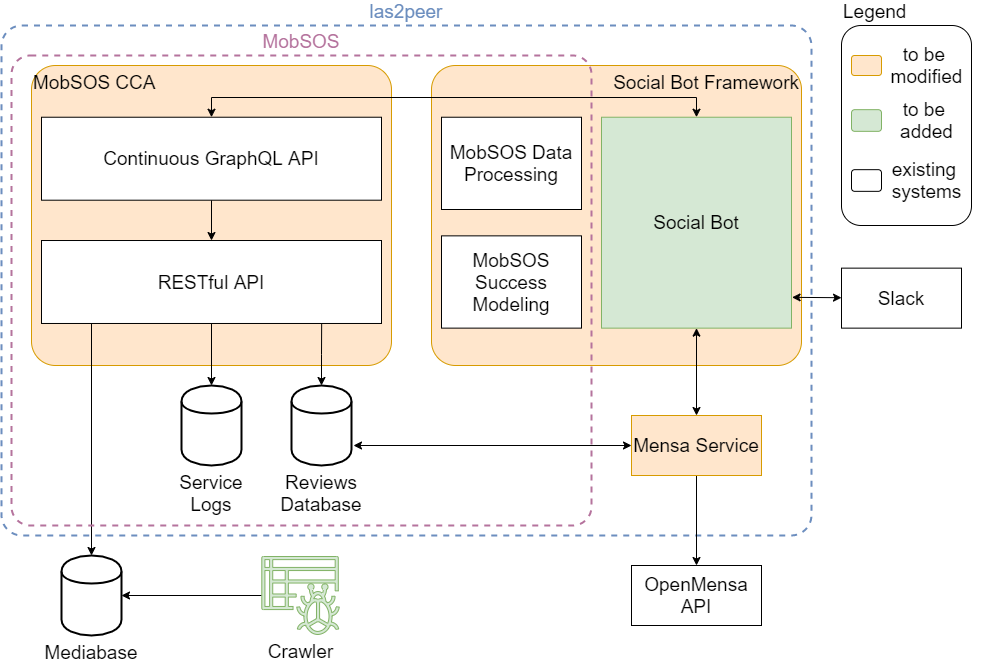
\includegraphics[width=\linewidth]{realization/components_overview.png}
  \caption{Overview of the different components}
  \label{fig:componentsOverview}
\end{figure}

\newpage

\section{Changes to Core Components} \label{sec:changes}

\subsection{Social Bot Framework}
The Social Bot Framework needs to be extended, such that the bot is able to listen to specific mentions in group chats and filtering out the rest of the conversations, such that the bot can be integrated in group chats, as a quiet agent.

A metion has the following form \texttt{@botname}, where \emph{botname} represents the username that the bot has in the Slack channel.

\subsubsection{Social Bot}
The Social Bot will be created, using the SBF frontend service.
The first feature, which will be implemented is quering the menu for a specific canteen. Next the review process will be implemented as a question-based dialogue. An example can be seen in figure \ref{fig:chatMockup}.
Both of these features should be implemented as soon as possible, to allow the collection of food review and such that the first phase of the evaluation can be done (see Chapter \ref{cha:eval}).
The food reviews will be done in private chat with the bot. The menu query should be available both in private chat and in channels, given that the SBF is already extended to allow for mentions.

The next feature, which will be implemented is the visualisation of success variables. Users should be able to formulate GraphQL queueries, which will be recognized by the bot to run the visualisations. Additionally, templates will be available, which are to be run when specific intents are recognized, such that the query visualisations can be done in an intuitive way. An example can be seen in figure \ref{fig:visualReq}.

Finally the success modeling will be implemented. Users should be able
to modify the success model in chat. Therefore, an update routine needs to be implemented, which is started at the recognition of a specific intent.

\subsection{MobSOS CCA}
The MobSOS CCA system needs to be extended such that the success model data can be visualized and sent as a picture to the user. Therefore, the Google Charts API will be used in combination with an HTML renderer, which will render the visualizations which were produced by the Charts API and send them back as a PNG to the Bot Service.

\subsection{Google Charts API}
Google Charts API\footnotemark is an API that provides visualizations for database data. The data, which should be visulaized needs to be wrapped inside a Javascript class called \texttt{DataTable}, which represents a two-dimensional table with rows and columns, where each column has a datatype.
A new column can be added using the \texttt{DataTable.addColumn} function, which takes the type and name as input. An example can be seen in Listing \ref{lst:gglCharts} from the Google Charts API documentation\footnotemark[\value{footnote}].

\begin{lstlisting}[caption=Example use of the DataTable class,captionpos=b,label={lst:gglCharts}]
var data = new google.visualization.DataTable();
data.addColumn('string', 'Topping');
data.addColumn('number', 'Slices');
data.addRows([
	['Mushrooms', 3],
	['Onions', 1],
	['Olives', 1], 
	['Zucchini', 1],
	['Pepperoni', 2]
]);
\end{lstlisting}

The visualizations are rendered as SVGs in the browser, but can be the PNG file can be accessed by maken an http call with the \texttt{getImageURI} as image URI parameter.

\footnotetext{\href{https://developers.google.com/chart}{Google Charts API}}

\subsection{GraphQL}
GraphQL\footnotemark is a query language specifation for web APIs.
\footnotetext{GraphQL: \href{https://graphql.github.io/}{https://graphql.github.io/}}
Instead of hitting multiple endpoints, like in standard REST APIs, for different requests, users can get all data from one endpoint, by specfifying the kind of data that they need as a query. This means that it prevents over- and underfetching of data.\footnotemark

\footnotetext{\href{https://www.howtographql.com/basics/1-graphql-is-the-better-rest}{https://www.howtographql.com/basics/1-graphql-is-the-better-rest}}

GraphQL does not mandate the use of a specific programming language, the actual implemtention is up to the developer of the server. \footnotemark
\footnotetext{\href{http://spec.graphql.org/June2018/}{http://spec.graphql.org/June2018/}}
Many different implemtentions have been written for programming languages like Java \footnote{Java GraphQL Library:\href{https://www.graphql-java.com/documentation/master/}{https://www.graphql-java.com/documentation/master/}} and Javascript. \footnote{Javascript GraphQL Library:\href{https://www.npmjs.com/package/express-graphql}{https://www.npmjs.com/package/express-graphql}}

Transforming an existing REST API into a GraphQL API can be a cumbersome task. An automation process in the form of a Wrapper has been proposed, which converts an existing schema such as a Swagger schema into a GraphQL schema\footnote{\href{https://github.com/yarax/swagger-to-graphql}{Swagger-to-GraphQL}}. Such a wrapper transforms GraphQL requests into RESTful requests as depicted in Figure \ref{fig:graphqlWrapper}.
\begin{figure}[h]
  \centering
  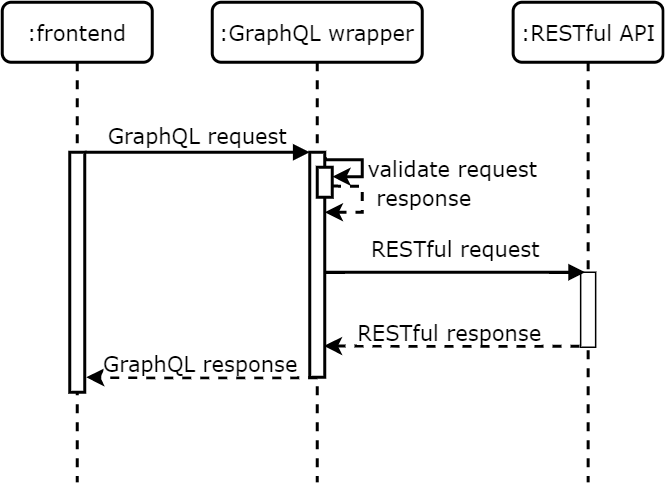
\includegraphics[width=0.6\linewidth]{realization/graphqlWrapper.png}
  \caption{Example use of community Service with the Bot}
  \label{fig:graphqlWrapper}
\end{figure}

In GraphQL, data objects are defined as a \emph{type}. GraphQL provides simple base-types like Int Float, Boolean and String, but new types can also be defined. An example can be seen in \ref{lst:GraphQLType}.
\begin{lstlisting}[caption={Example of a GraphQL schema},captionpos=b,label={lst:GraphQLType}]
type Review {
  id: ID
  rating: Int
  description:String
}
\end{lstlisting}
New fields can be dynamically added without influencing existing queries. The schemas are formalized as either a \emph{Query }, or a \emph{Mutation}. They are declared by the keyword \emph{schema}. The query keyword can be omitted. An example of a query can be seen in listing \ref{lst:GraphQLQuery}.
\begin{lstlisting}[caption={Example of a GraphQL Query},captionpos=b,label={lst:GraphQLQuery}]
{
  Review(id: "1000") {
    rating
  }
}
\end{lstlisting}
Here we access the rating of the review with the ID 1000.

Mutations are used to modify data. An example of a query can be seen in listing \ref{lst:GraphQLMut}.
\begin{lstlisting}[caption={Example of a GraphQL Mutation},captionpos=b,label={lst:GraphQLMut}]
mutation addReview(){
  {
	rating 
	description
  }
}
\end{lstlisting}

\begin{figure}[h]
  \centering
  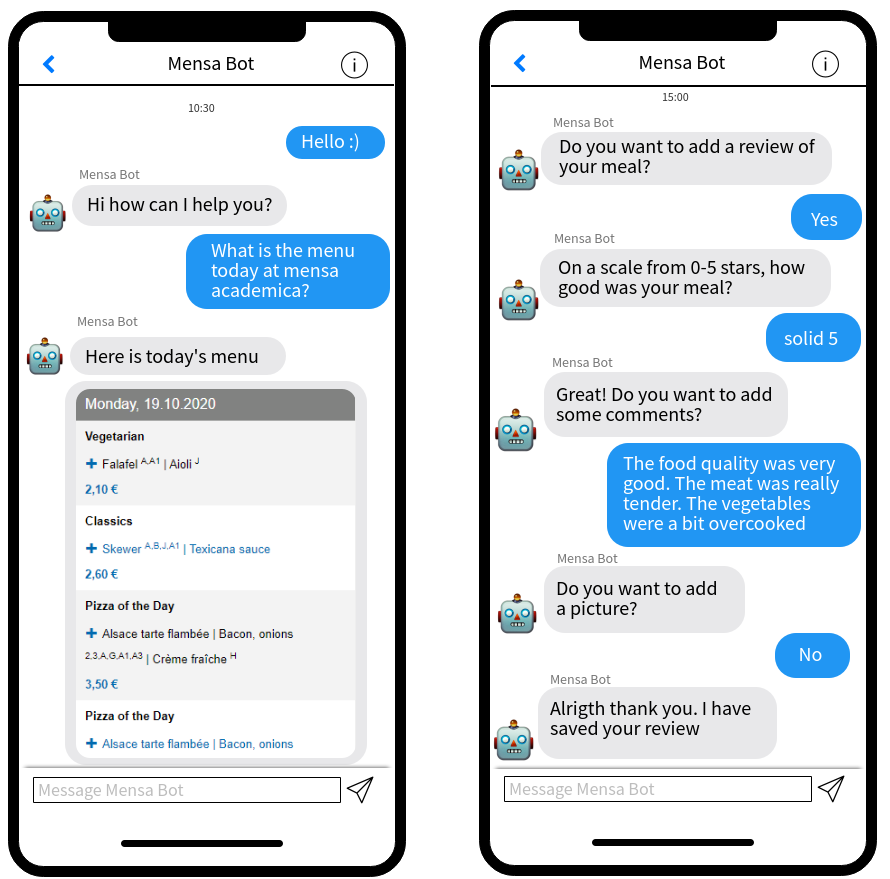
\includegraphics[width=0.8\linewidth]{realization/chat_mockup.png}
  \caption{Example use of community Service with the Bot}
  \label{fig:chatMockup}
\end{figure}

\begin{figure}[h]
  \centering
  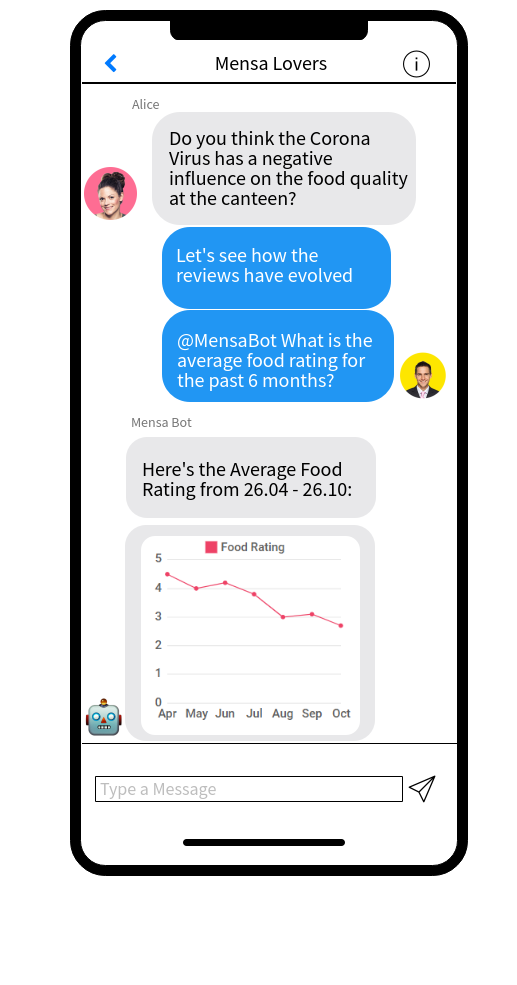
\includegraphics[width=0.35\linewidth]{realization/visual_req.png}
  \caption{Example of a chat interaction with the Bot}
  \label{fig:visualReq}
\end{figure}